% ---------------------------------------------------
% ----- Introduction of the template
% ----- for Bachelor-, Master thesis and class papers
% ---------------------------------------------------
%  Created by C. Müller-Birn on 2012-08-17, CC-BY-SA 3.0.
%  Last upadte: C. Müller-Birn 2015-11-27 
%  Freie Universität Berlin, Institute of Computer Science, Human Centered Computing. 
%
\chapter{Introduction}
\label{chap:introduction}

\section{Project IKON}

This thesis has a direct application in a project which tries to explore potentials for knowledge transfer activities at a research museum. Project \textit{IKON} was started in cooperation with the German Natural History Museum in Berlin which houses more than 600 \tk{Right number?} scientists, PhD students and other staff. With that size of scientific staff the institution is a global player in research on evolution and biodiversity \cite{IntroducingMuseumFur}. Despite its importance in the research landscape the museum is challenged with a lack of shared knowledge across working groups and organizational structures such as departments. In interviews researchers from the project were able to trace these problems back to the very intricate and complex layout of rooms and halls in the building which was originally constructed in 1810. In order to mitigate this problem \autoref{pic:IKON-clusterview} shows one of the main deliverables of \textit{IKON} - a ML-driven data visualization which follows the path of knowledge at this research museum from its creation in projects over knowledge transfer activities, where multiple projects exchange their findings and try to generate added value for each other, to the final target group. Knowledge transfer is made explicitly visible by showing projects not in the predefined taxonomy of the museum, but instead in semantic relation to each other. This is accomplished by running all project abstracts through a topic extraction pipeline consisting of four major components, as seen in \autoref{pic:general_topic_extraction_pipeline}.  

\begin{figure}[t]
	\centering
	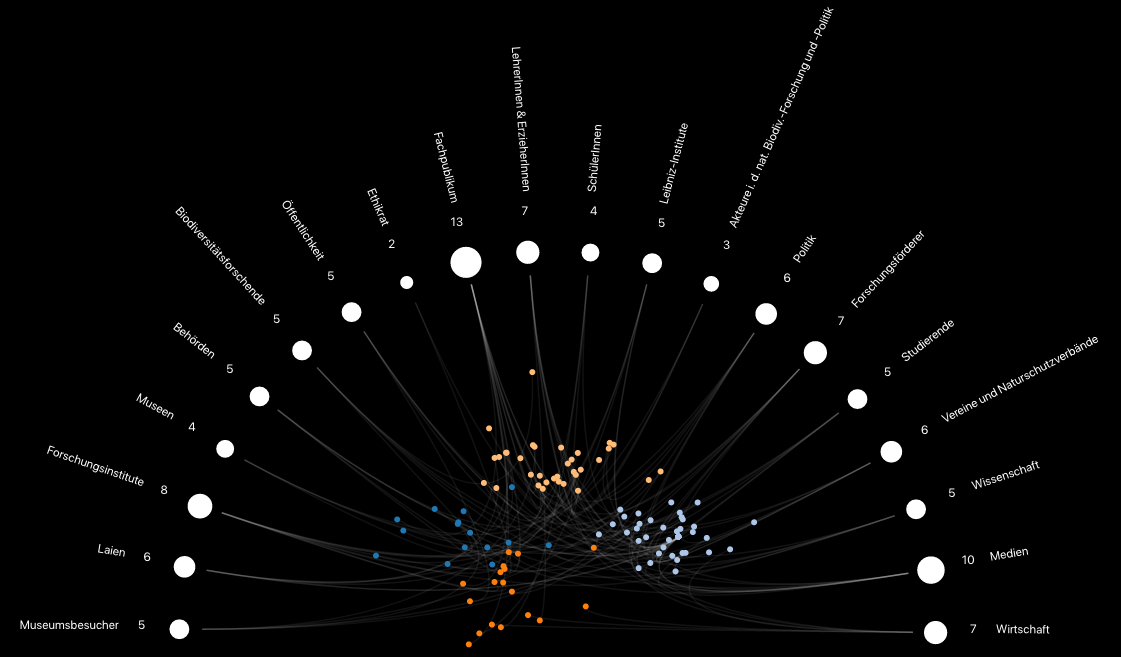
\includegraphics[width=400px]{../chapters/introduction/graphics/ikon-clusterview}
	\caption{\label{pic:IKON-clusterview} BPMN process diagram of the existing topic extraction pipeline}
\end{figure}

% Define block styles
\tikzstyle{decision} = [diamond, draw, fill=blue!20, 
text width=4.5em, text badly centered, node distance=3cm, inner sep=0pt]
\tikzstyle{block} = [rectangle, draw, fill=blue!20, 
text width=5em, text centered, rounded corners, minimum height=4em]
\tikzstyle{line} = [draw, -latex']
\tikzstyle{cloud} = [draw, ellipse,fill=red!20, node distance=3cm,
minimum height=2em]

\begin{figure}[t]
	\centering
	\begin{tikzpicture}[node distance = 4cm, auto]
	% Place nodes
	\node [block] (emb) {Document embedding};
	%\node [cloud, left of=emb] (expert) {expert};
	%\node [cloud, right of=emb] (system) {system};
	\node [block, right of=emb] (topic) {Topic extraction};
	\node [block, right of=topic, above of=topic] (cluster) {Clustering};
	\node [block, right of=topic, below of=topic] (2D) {Reduction into 2D};
	% Draw edges
	\path [line] (emb) -- (topic);
	\path [line] (topic) -- (cluster);
	\path [line] (topic) -- (2D);
	%\path [line] (identify) -- (evaluate);
	%\path [line] (update) |- (identify);
	%\path [line,dashed] (system) |- (evaluate);
	\end{tikzpicture}
	\caption{\label{pic:general_topic_extraction_pipeline} Components of a general unsupervised topic extraction pipeline}
\end{figure}

First user tests and interviews unveiled that, even though the visualization was specifically tailored to non-technical users \tk{neeeds definition}, the scientists from the museum had a hard time interpreting and understanding the output generated by the pipeline.  Based on these findings and a workshop with the main researchers of project \textit{IKON} I was able to extract a set of questions that a subject tries to answer while interacting with the visualization:

\begin{enumerate}
	\item How does the research landscape look like and on what kind of topics are prominent?
	\item What does a cluster mean?
	\item What does the distance between clusters/projects mean?
	\item How similar are two projects/clusters?
\end{enumerate}

\section{Interpretability}

\tk{Interpretation of machine learning (ML) results is a major challenge for humans, especially for non-technical experts [ref]. Research on interpretability\footnote{Which we position to be a high-level precondition for Explainability from the XAI \cite{gunning_broad_2016} and Fairness, Accountability and Transparency, from the FAT-ML discourse \cite{kohli_translation_2018}.} in the ML community has focused on developing interpretability techniques, i.e. specific technical approaches to generate explanations\footnote{Which we define as instances of interpretability techniques.} for ML results. However, applications of these techniques are predominantly concerned with making particular model features understandable, rather than supporting the interpretation of ML-driven systems in a specific context of use. At the same time, research in the HCI domain often remains on a formal, algorithmic level---explanations tend to be technical and tailored to an expert audience, mirroring the technical focus of ML research. Realistic use cases and qualitative, context-aware evaluations to inform the selection and design of interpretability techniques remain rare. 
While we do not see complete transparency as a prerequisite for interpretability we hypothesize that in general, since interpretation is dependent on context, interpretability techniques cannot be fully context agnostic either. Therefore, our general approach is to research interpretability from a context-aware perspective, i.e. we explore how interpretability can be operationalized in a specified, well-defined domain context.}

